\chapter{Linked List}


\section{Operations}
\subsection{Fundamentals}
Get the $pre$ reference:
\begin{python}
dummy = Node(0)
dummy.next = head
pre = dummy
cur = pre.next
\end{python}

In majority case, we need a reference to pre.

\subsection{Basic Operations}
\begin{enumerate}
\item Get the length
\item Get the $i$-th object
\item Delete a node 
\item Reverse
\begin{figure}[]
\centering
\subfloat{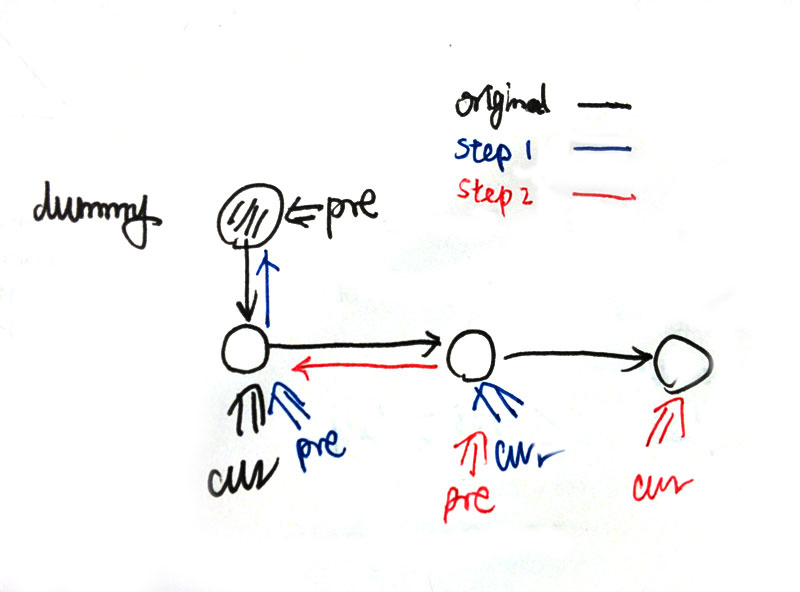
\includegraphics[scale=1.0]{ll_reverse}}
\caption{Reverse the linked list}
\label{fig:LABEL}
\end{figure}
\begin{python}
def reverseList(self, head):
    dummy = ListNode(0)
    dummy.next = head

    pre = dummy
    cur = pre.next
    while pre and cur:
        nxt = cur.next
        # left to right eval for multi-assignment7
        cur.next = pre
        pre, cur = cur, nxt

    dummy.next.next = None  # original head
    return pre  # new head
\end{python}
Notice: the evaluation order for the swapping the nodes and links. 
\end{enumerate}

\subsection{Combined Operations}
In $O(n)$ without extra space:
\begin{enumerate}
\item Determine whether two lists intersects
\item Determine whether the list is palindrome 
\item Determine whether the list is acyclic
\end{enumerate}

\section{Combinations}
\subsection{LRU}
Core clues:
\begin{enumerate}
\item Ensure $O(1)$ find $O(1)$ deletion. 
\item Doubly linked list + map.
\item Keep both \pyinline{head} and \pyinline{tail} pointer.
\item Operations on doubly linked list are case by case.  
\end{enumerate}
\begin{python}
class Node(object):
    def __init__(self, key, val):
        self.key = key
        self.val = val
        self.pre, self.next = None, None


class LRUCache(object):
    def __init__(self, capacity):
        self.cap = capacity
        self.map = {}  # key to node
        self.head = None
        self.tail = None

    def get(self, key):
        if key in self.map:
            cur = self.map[key]
            self._elevate(cur)
            return cur.val

        return -1

    def set(self, key, value):
        if key in self.map:
            cur = self.map[key]
            cur.val = value
            self._elevate(cur)
        else:
            cur = Node(key, value)
            self.map[key] = cur
            self._appendleft(cur)

            if len(self.map) > self.cap:
                last = self._pop()
                del self.map[last.key]

    # doubly linked-list operations only
    def _appendleft(self, cur):
        """Normal or initially empty"""
        if not self.head and not self.tail:
            self.head = cur
            self.tail = cur
            return

        head = self.head
        cur.next, cur.pre, head.pre = head, None, cur  # safe
        self.head = cur

    def _pop(self):
        """Normal or resulting empty"""
        last = self.tail
        if self.head == self.tail:
            self.head, self.tail = None, None
            return last

        pre = last.pre
        pre.next = None
        self.tail = pre
        
        return last

    def _elevate(self, cur):
        """Head, Tail, Middle"""
        pre, nxt = cur.pre, cur.next
        if not pre:
            return
        elif not nxt:
            assert self.tail == cur
            self._pop()
        else:
            pre.next, nxt.pre = nxt, pre  # safe

        self._appendleft(cur)
\end{python}
